The measurements of $R_K$ and $R_{K^*}$ in the low $q^2$ 
and central $q^2$ regions currently represent the most 
precise tests of LFU. 
Contrary to previous measurements, this analysis aligns 
with the SM predictions, with an agreement of 
$\num{0.2}\sigma$, as shwon in figure \ref{fig:results}. 
This study underscores the importance of understanding 
electron misidentification and also demonstrates the 
benefits of a double-ratio approach in minimizing 
systematic uncertainties. The statistical uncertainties 
significantly outweigh the systematic uncertainties in this 
analysis, suggesting that a larger dataset is required 
to improve the precision of the measurement.

\begin{figure}
    \centering
    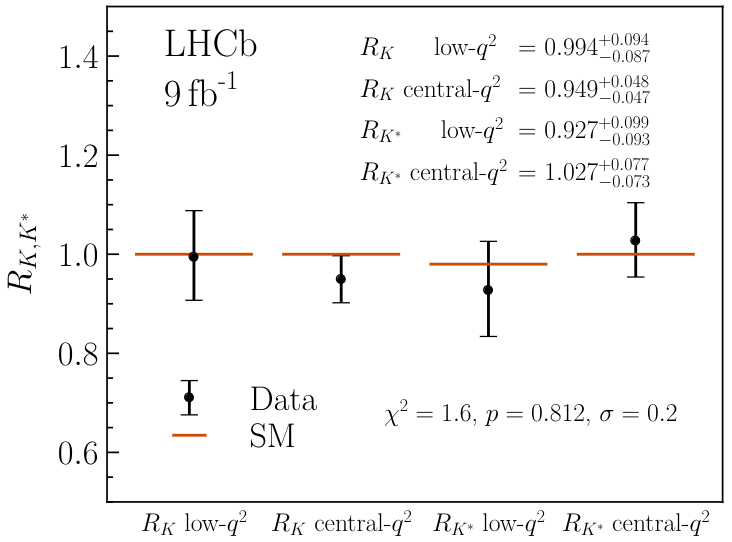
\includegraphics[width=\linewidth]{figures/results.png}
    \caption{Graphical comparison of the measured results of $R_K$ and $R_{K^*}$ in the low and central $q^2$ range with the SM predictions \cite{lhcbcollaboration2022measurement}.}
    \label{fig:results}
\end{figure}

While the LFU tensions with respect to the SM 
appear to be of systematic origin, the tensions related to 
the branching fractions $\mathcal{B}(B^{(0,+)}\to K^{(+,*0)}\ell^+\ell^-)$ 
remain \cite{Branchingfraction}.

With the upcoming LHCb Run 3 offering increased luminosities 
and track multiplicities, significant upgrades to the subdetectors 
and trigger system have been made. These improvements are expected 
to further refine the precision of Lepton Flavor Universality tests.